\chapter{Megvalósítás}

\section{Aréna}
\subsection{Prototípus}
Az aréna több fázison ment karesztül a játék fejlesztése során.
Először egy prototípust készíttem el azért hogy az elrendezés és az arányok átláthatóak legyenek. Tervezés során fontos volt a szimertia illetve az hogy ne legy túl zsúfolt a játéktér.

\begin{figure}[h]
        \centering
        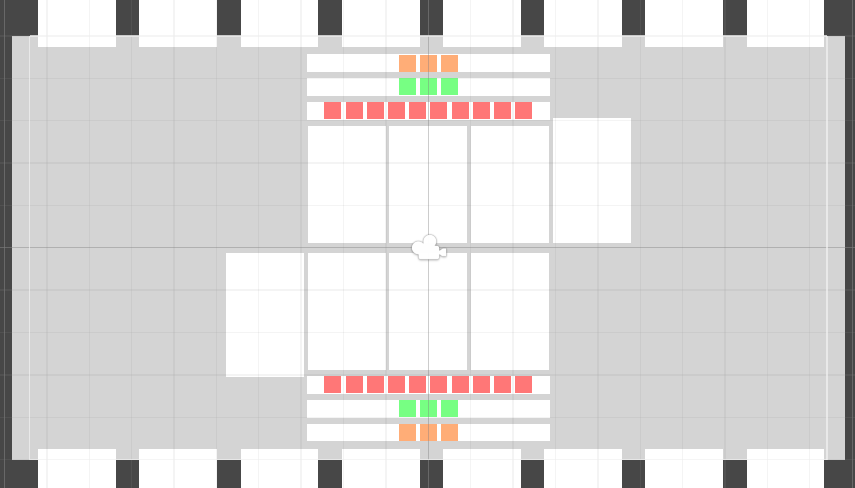
\includegraphics[width=400px,keepaspectratio]{images/proto.png}
        \label{Proto}
        \caption {Aréna prototípus}
    \hspace{1em}
\end{figure}

Ebben a fázisban a pálya már átlátható volt viszont még semmilyen funkció nem élt és az elrendezés kézzel történt. A későbbi verziókban történő változások ennek a ténynek tudhatóak be, mivel itt még nem rendereljük dinamikusan a képernyő elemeke ( az élet pontokat, akció- és reakció pontokat stb). Ez a későbbiekben Unity-n belül használható layoutok segítségével fogjuk megoldani.

\clearpage

\subsection{Első verzió}

\begin{figure}[h]
        \centering
        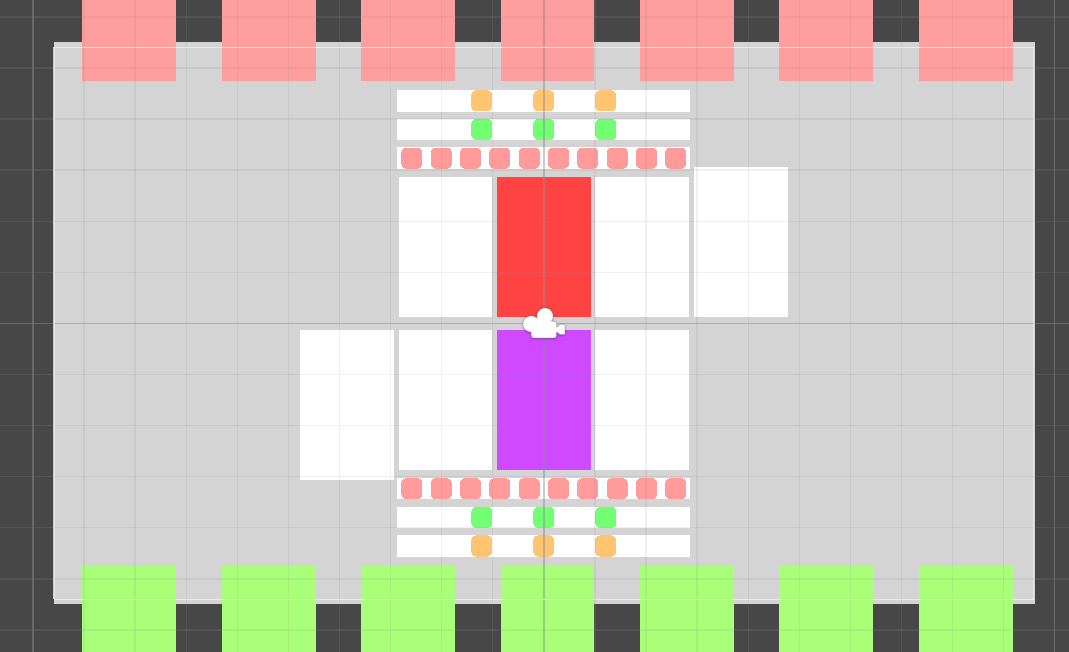
\includegraphics[width=400px,keepaspectratio]{images/Boardconcept.png}
        \label{ArenaLvl2}
        \caption {Aréna prefab-ekkel}
    \hspace{1em}
\end{figure}

Ebben a fázisban a kézzel elhelyezett elemeket átvették a layoutok és a prefabok. A már előbb említett layaoutok egy konzisztens elhelyezkedést garantálnak az elemeknek. Felmerülhet a kérdés hogy mik is azok a prefabok. A prefabok olyan játék objektumok amik le vannak mentve mint egy összeszerelt entitás. Megtudjuk határozni ennek a tulajdonságai és a rajta lép scripteket előre. Így mikor létre akarunk hozni egy játék objectumot akkor elég csak ezt a prefabot meghívni. A fenti ábrán látható: kártyák, élet pontok, akció pontok, és reakció pontok mind a játékos mind az ellenfél oldalán prefabokat használnak.


\clearpage

\subsection{Második Verzió}

A következő lépésben hozzá adtuk az End Turn gombot és a Karakter képét. Ezen felül a kézben lévő kártyákat generáljuk ahelyett hogy csak előre bele lennének helyezve a layoutba. A Felszerelés kártyák teszetlésének érdekében ideiglenesen bekerült egy extra kártya hely.

\begin{figure}[h]
        \centering
        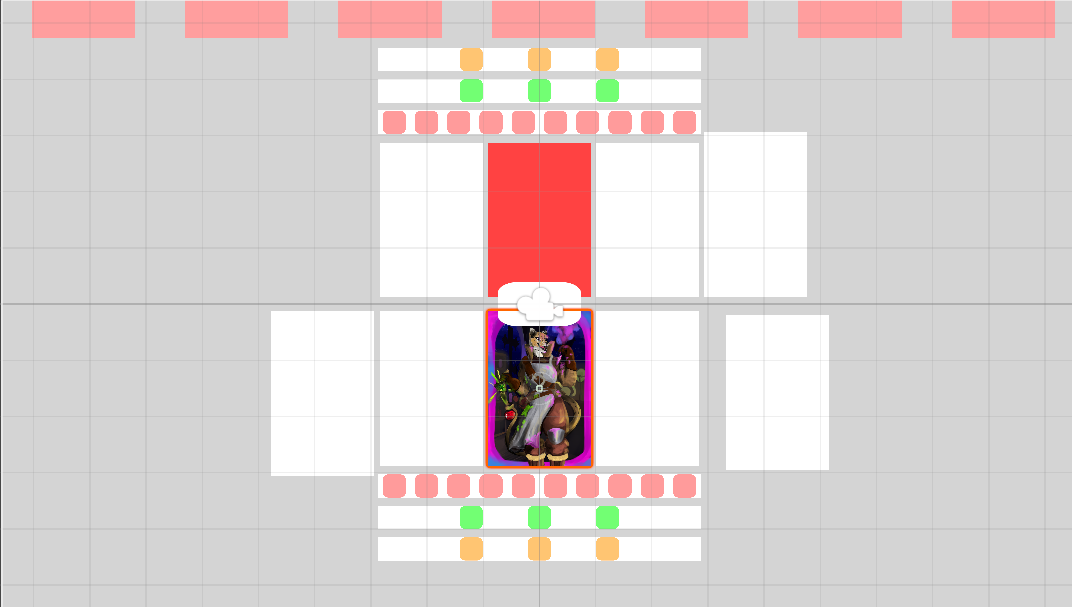
\includegraphics[width=400px,keepaspectratio]{images/board1.png}
        \label{ArenaLvl3_v1}
        \caption {Aréna futtatás előtt a kézzel berakott elemekkel}
    \hspace{1em}
\end{figure}
\begin{figure}[h]
        \centering
        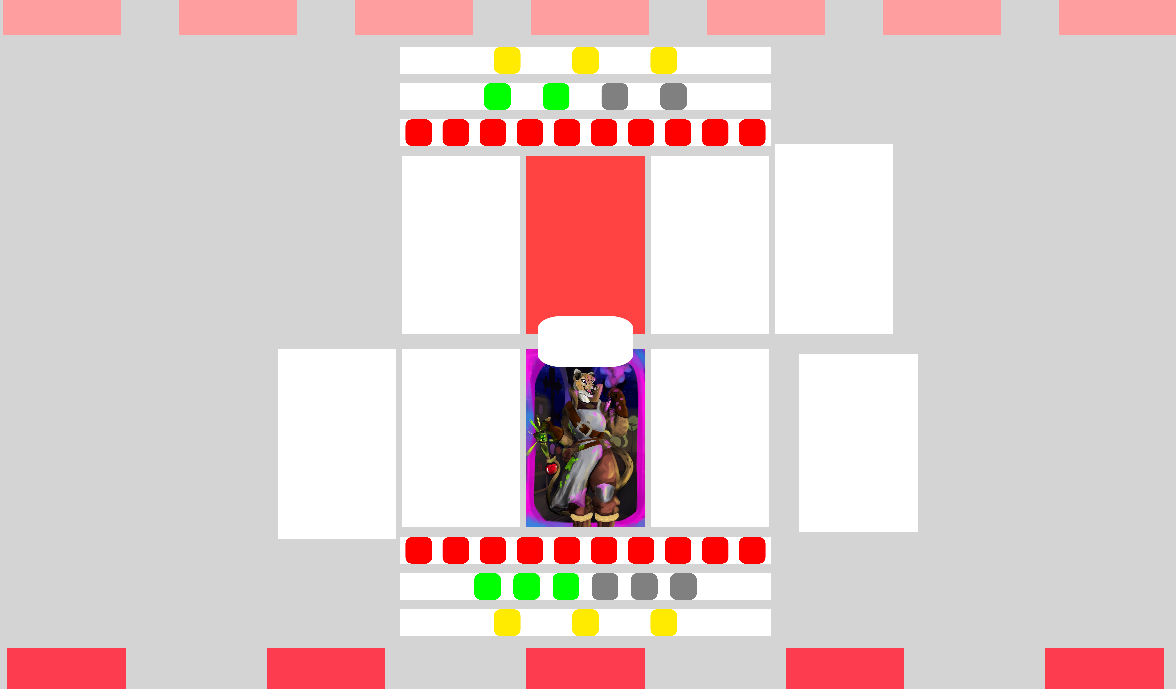
\includegraphics[width=400px,keepaspectratio]{images/board2.png}
        \label{ArenaLvl3_v2}
        \caption {Aréna futtatás után a generált elemekkel}
    \hspace{1em}
\end{figure}

\clearpage

\subsection{Végső Verzió}
Ez után az aréna végső stáduimba lépett. Az élet pontok át lettek formázba egy kicsit és a számuk meg lett növeltve 10->20. Az ideiglenes kártya hely ki lett véve. A játékos kártyáit mostmár a játékos paklija alapján, abból generálja a játék. Az élet csíkon a bal oldalra be lett helyezve egy mutató ami a pajzs értéket mutatja, a jobb oldalon pedig egy másik mutató ami pedig az élet pontokat mutatja. Ez az ellenfél oldalon is bekerült. Az End Turn gomb is kapott egy feliratot illetve zöld színű lett hogy jelezze hogy a játékos kezd.

\begin{figure}[h]
        \centering
        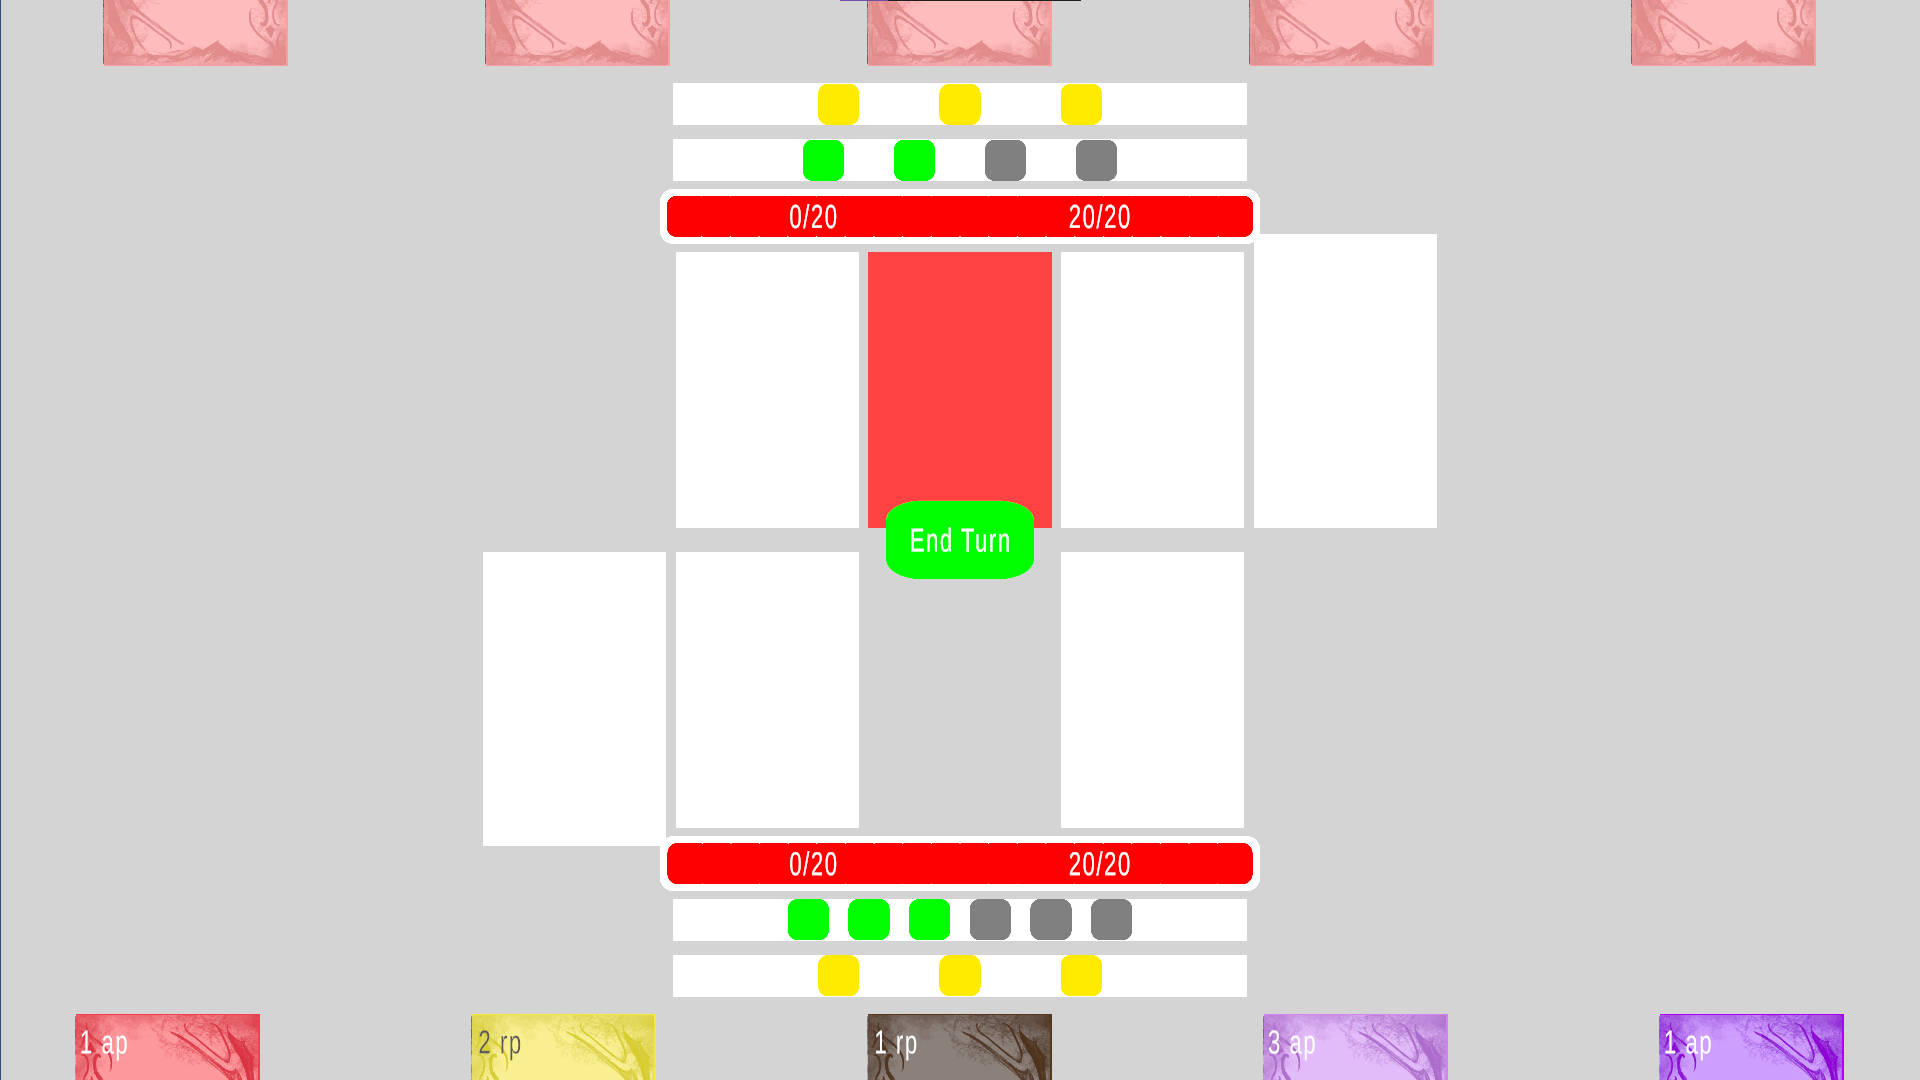
\includegraphics[width=400px,keepaspectratio]{images/image.png}
        \label{ArenaFinal}
        \caption {Aréna végső fázisban}
    \hspace{1em}
\end{figure}

Ez a verzió fogad minket amikor elkezdünk játszani.

\clearpage

\section{Kártya Húzás}
\subsection{Scriptable objects}
A karakterek információ (élet pontok, bónus sebzés, stb) egy-egy scriptable objectbe vannak letárolva. Ezek olyan játék objectumok amelyek információt tárolnak. Írthatóak és olvashatóak. Nagyon hasznosak mivel így van egy előre elkészített struktúra ami le tudja tárolni egy adott típusú objectum információit.
\\\
\begin{lstlisting}[language=CSharp,style=CSharpBase,caption={A Klass Scriptable Object kódja}]
using System.Collections;
using System.Collections.Generic;
using UnityEngine;

public enum Classes
{
    Warrior, Ranger, Necromancer,Paladin,Alchemist,Ninja,Druid,Mage
}

public enum WeaponTypes 
{
    Melee,Ranged,Magic,Summon
}

[CreateAssetMenu(menuName = "KlassData")]
public class ClassDataSo : ScriptableObject
{

    public int maxHp;
    public int currentHp;
    public int shield;
    public int maxAp;
    public int currentAp;
    public int apRegain;
    public int maxRap;
    public int currentRap;
    public int attackDmgBonus;
    public int spellDmgBonus;
    public Sprite sprite;
    public Classes characterKlass;
    public WeaponTypes weapon;
    public GameObject prefab;
    public List<CardDataSo> baseDeck;
    public List<CardDataSo> deck = new();
}
\end{lstlisting}

\clearpage

\subsection{A húzás működése}
Amikor a játékot elíndidjuk a karakter SO-jéból (Scriptable Object) kivesszük az alap paklit. Ezt behejezzük a játékon belül használt pakliba. Ez a pakli fog változni amikor kártyát húznuk illetve amikor kártyát vissza teszünk. A pakli egy lista ami a benne lévő kártyák információját tárolja. A kártyák egy másik SO-ba vannak letárolva. Kártya húzáskor ezt a kártya SO-t inicializáljuk az az egy fizikai játék objectumként hozunk létre.
Még mielőtt a kártya létrejöhetne meg kell nézzük hogy belefér e a játékos kezébe. Ha nem akkor a húzás nem történik meg. Ha igen akkor a kártyának a vizuális elemeit frissítjük (Ára, neve, típusa, stb). Miután ez megtörtént létrehozzuk az objectumot és megadjuk neki hogy melyik kártya SO hozta létre. Ez a fizikai objectum lesz majd kijátszható a játékos által.
\\\
\begin{lstlisting}[language=CSharp,style=CSharpBase,caption={A kártya kézbe helyezése}]
public void PutCardInHand()
{
    if (deck.Count == 0 || hand.childCount >= 10)
    {
        return;
    }
    var data = deck[0];
    if (data.isActionCost)
    {
        data.prefab.transform.Find("price").GetComponent<TextMeshPro>().text = 
        string.Concat(data.cost) + " ap";
    }
    else
    {
        data.prefab.transform.Find("price").GetComponent<TextMeshPro>().text = 
        string.Concat(data.cost) + " rp";
    }
    data.prefab.transform.Find("Desc").GetComponent<TextMeshPro>().text =
    string.Concat(data.description);
    
    data.prefab.transform.Find("dmg").GetComponent<TextMeshPro>().text = 
    string.Concat(data.dmg);
    
    data.prefab.transform.Find("Type").GetComponent<TextMeshPro>().text = 
    string.Concat(data.cardType);
    
    var card = Instantiate(data.prefab, hand);
    card.GetComponent<Card>().data = data;
    deck.Remove(deck[0]);
}
\end{lstlisting}
\clearpage
\section{Kártya Kijátszás}
A kártyák kijátszása a Unity ActionHandler system-ével működik. Ez az event system úgy működik hogy van egy event stack. Erre a stackre iratkoznak fel az egyes metódusok. És amikor invoke-oljuk ezt a stacket az összes metódus meghívódik ami feliratkozott. Ezek a metódusok nem törlődnek amikor a stack meghívásra kerül.
\\\
\begin{lstlisting}[language=CSharp,style=CSharpBase,caption={Event kezelő}]
using System.Collections;
using System.Collections.Generic;
using UnityEngine;

public class CardAction : MonoBehaviour
{
    public delegate void ActionHandler();
    public ActionHandler onCardPlayed;
    CardDataSo data;
    void Start()
    {
        data = GetComponent<Card>().data;
    }

    public void PlayCard() 
    {
        onCardPlayed?.Invoke();
        if (GameManager.instance.heroData.currentAp >
                                GameManager.instance.heroData.maxAp 
            || GameManager.instance.heroData.currentHp >
                                GameManager.instance.heroData.maxHp)
        {
            GameManager.instance.heroData.SetToMax();
        }
    }  
}
\end{lstlisting}

\section{Mesterséges inteligencia}
Annak köszönhetően hogy a játék egyszemélyes szükség van egy ellenfélre aki ellen a játékos tud játszani. Az ellenség egy egyszerű mesterséges inteligenciát alkalmaz. Képes támadni, gyógyítani magán, pajzsot adni magának, felszerelést lehelyezni illetve 5 lappal kezdi mindegy egyes körét. 

Ezeken felül hogy a játék egyre nehezedjen ahogy haladunk előre az ellenfél minden új csata folyamán kap 5 plusz életpontot, minden 3. kör alkalmával pedig plusz 1 akció- és reakció pontot, plusz egy akció pontot nyer vissza körönként és plusz 1 kártyát kap körönként.

%Diagrammok és folyamat ábrák
%másjátékokkal valú összahasonlítás (összehasonlító táblázat)
%